\documentclass[aps,letterpaper,11pt]{revtex4}

\usepackage{graphicx}
\usepackage{float}
\usepackage{verbatim}
\usepackage{amsmath}
\usepackage{amssymb}

\newcommand{\labno}{10}
\newcommand{\labtitle}{Calculating the Maximum Stretched Length of a "Bungee Cord" for the \textit{Leap of Faith Bungee Jumping Company}}
\newcommand{\authorname}{Kevin Truong}
\newcommand{\professor}{Dr. Melanie Lutz}
\newcommand{\classno}{Physics 006}
\newcommand{\labpartners}{Sean Casey, Kevin Castillo, and Dulce Payan}
\newcommand{\submitdate}{May 2,2017}

\begin{document}

\begin{titlepage}
\begin{center}
\hspace{-136mm}\boxed{{\Large \textsc{Lab No. \labno}}}\\\vspace{30mm}
{\Large \textsc{\labtitle} \\ \vspace{4pt}}
\rule[13pt]{\textwidth}{1pt}\\ \vspace{150pt}
{\large By: \authorname \\ \vspace{10pt}}
Lab Partners: \labpartners \\
Instructor: \professor \vspace{10pt} \\
Solano Community College\\ \classno \\ \vspace{10pt}
\submitdate
\end{center}
\end{titlepage}

\section{Abstract}

This experiment used Hooke's law and the conservation of energy in a system to calculate the height that a mass, attached to a support by rubber bands, so the mass lightly taps a box. Looking at the linear graph(Force vs. Length) that models Hooke's law on the rubber bands, the slope of the linear line was the k value of the rubber bands; which was founded to be 17.708$\frac{N}{M}$. Then the linear equation of the trendline from the Force vs. Time graph was used to find the equilibrium length with the mass attached, by setting the linear equation y=17.708x+8.901 equal to zero. The eqquilibrium length, $y_0^*$, was 0.5612m. 

Using the conservation of energy in the system where state one had only gravitational potential energy because the mass started at some height away from the origin and state two only had elastic potential energy because the rubber band was at maximum stretch and was at origin, and all of the values found in the experiment, the $y_f$ so that the mass lightly taps the box was 0.872m. This resulted in a successful run, we dodged the ground on the first drop and lightly tapped the box on the second drop! 

\section{Introduction}

To a certain extent, springs and rubber bands follow the properties of Hooke's law, also known as $F = -k \Delta x$, where the force on the body by the spring is equal to the spring constant of the particular spring/rubber band times the compressed or stretched length relative to the equilibrium length. 

When analyzing a spring with some spring constant, k, the increase and decrease in the force of the spring is directly proportional to the stretched or compressed length of the spring relative to the equilibrium length. In this experiment, the rubber bands analyzed have a spring constant, k, that was found by analyzing the Force Vs. Length graph of the system. 

In the experiment conservation of energy was also analyzed at two stages, when there was only gravitational potential energy in the body, and when there was only elastic potential energy in the body. 

\section{Experimental Details}

Equipment for this experiment includes 8 rubber bands, a tall support, a meter stick, multiple masses, a table, and a computer. The 8 rubber bands acted as the bungee cord and were intertwined to make a better representation, it was connected to the tall support. The tall support was connected to the table and was hanging over the edge of the table, to simulate the system of a bungee jump. A meter stick was used to measure lengths of objects, the multiple masses were used to test the stretch of the rubber bands and collect data about the rubber bands. The table was used to anchor the tall support. The computer was used to organize the data collected using the meter stick.  

The experiment explored was distance $y_f$ the tall support needed to raised or lowered relative to the floor, so the 100 gram mass wouldn't hit the floor and would lightly tap the box, simulating a Bungee Jump off a bridge and lightly tapping the water. It was important to take certain things into account, for example the elasticity of the rubber band would degradate after multiple amounts of uses, so it was necessary and important to keep the stretching of the rubber bands to a minimum. It's also important to note that the measuring and collecting data occured with the use of a meter stick, so it's necessary to be very precise in the "eye-balling" of the values. 

\begin{center}
\underline{Diagram 1}\\
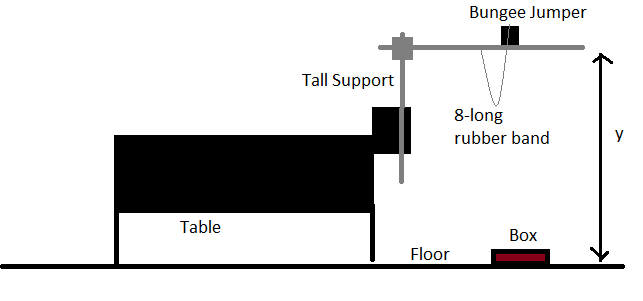
\includegraphics[width = 4in]{Setup.png}\\
\textit{Diagram 1: Setup For the Bungee Jump}\\
\end{center}

\newpage

\begin{center}
\underline{Diagram 2}\\
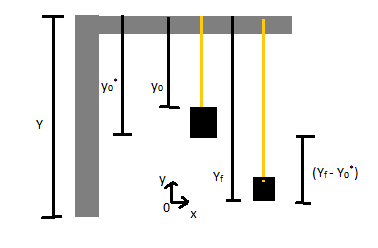
\includegraphics[width=4in]{Notations.png}\\
\textit{Diagram 2: the Notations of the experiment}
\end{center}

\section{Results and Analysis}

\subsection{Solving for $y_f$, Theoretically}

To solve for the maximum stretched length of any bungee cord, or in this case the rubber band it is necessary to analyze the energy in the system as the object falls from some height at rest and reaches the maximum stretched length. At these two points the velocity of the mass is zero. Let the origin be at the point of maximum stretched length. In state one, when the object is at rest and is about to be dropped, the object only has gravitational potential energy because the object's velocity is zero, there is no "tug" on the rubber band so there is no elastic potential energy, and the object is a distance of $y_f$ away from the origin. 

In the second state of the object, there is only elastic potential energy because the rubber band is stretched some distance. There is no kinetic energy at state two because the velocity at maximum stretch is zero because it's beginning to bounce back up towards the rubber band's equilibrium length. There is also no gravitational potential energy in state two because the object is at the origin, so there is no height or distance away from the origin. 

Therefore the object's energy can be written when comparing state one and state two as:

$$ mgy_f= \frac{1}{2}k \Delta y^2$$

where $y_f$ is the distance from the initial position to the maximum stretched length, k is the "spring" constant of the rubber band, and $\Delta y$ is the change in the equilibrium length($y_0^*$) and the maxed stretched length($y_f$).

$$ \therefore mgy_f= \frac{1}{2}k(y_f - y_0^*)^2$$

After expanding and simplifying the equation to get all values onto one side, it is easy to see that the equation will be quadratic:

$$ \therefore ky_f^2-2y_f(mg+ky_0^*) + ky_0^{*2} = 0$$

This means that $y_f$ can be solved using the quadratic equation where $a = k$, $b=-2(mg+ky_0^*)$, and $c=ky_0^{*2}$.

\subsection{Obtaining the value for k}

To find the value of k of the rubber band, it is necessary to look at Hooke's Law that states:

$$ F=k \Delta x$$

where F is the force of the spring, k is the spring constant, and $\Delta x$ is the stretched spring(rubber band) relative to the equilibrium length.

Solving for k:

$$ k = \frac{F}{\Delta x}$$

This means that if a known mass is attached to the rubber band and the stretched length is collected, k can be found. For an accurate calculation of the k value, multiple masses can be placed onto the rubber band and the stretches can be measured using a meter stick, where all the data can be placed into Excel and a graph can be created comparing the force and the stretched length; which will result in a linear line and the slope of this linear line will be the value of k. This can be easily seen when analyzing Hooke's law, $F=k \Delta x$ which is a linear equation with k being the slope of the linear line created by the equation.

In the experiment multiple masses were connected to the rubber band and the stretched lengths were all measured using a meter stick. The masses that were used were 5g,10g, 20g, 30g, 40g, 50g, 60g, 70g, 80g, 90g, and 100g.  
\newpage

\begin{center}
\underline{Table:}\\
\begin{tabular}{|c|c|c|c|}
\hline
l(cm) & m(g)& l(m)& F(N)\\
\hline
50.5 & 5 & 0.505 & 0.049\\
\hline
51 & 10 & 0.51 & 0.098\\
\hline
51.6 & 20 & 0.516 & 0.196\\
\hline
52.1 & 30 & 0.521 & 0.2943\\
\hline
52.4 & 40 & 0.524 & 0.3924\\
\hline
53 & 50 & 0.53 & 0.4905\\
\hline
53.5 & 60 & 0.535 & 0.5886\\
\hline
54 & 70 & 0.54 & 0.6867\\
\hline
54.5 & 80 & 0.545 & 0.7848\\
\hline
55.5 & 90 & 0.555 & 0.8829\\
\hline
56 & 100 & 0.56 & 0.981\\
\hline 
\end{tabular}
\\
\vspace{5mm}
\textit{The data collected from the multiple hanging masses}
\end{center}

The lengths in meters and the forces in Newtons were then plotted to create a Force vs. Length graph, shown in figure one.

\newpage

\begin{center}
\underline{Figure 1}\\
\vspace{-50mm}
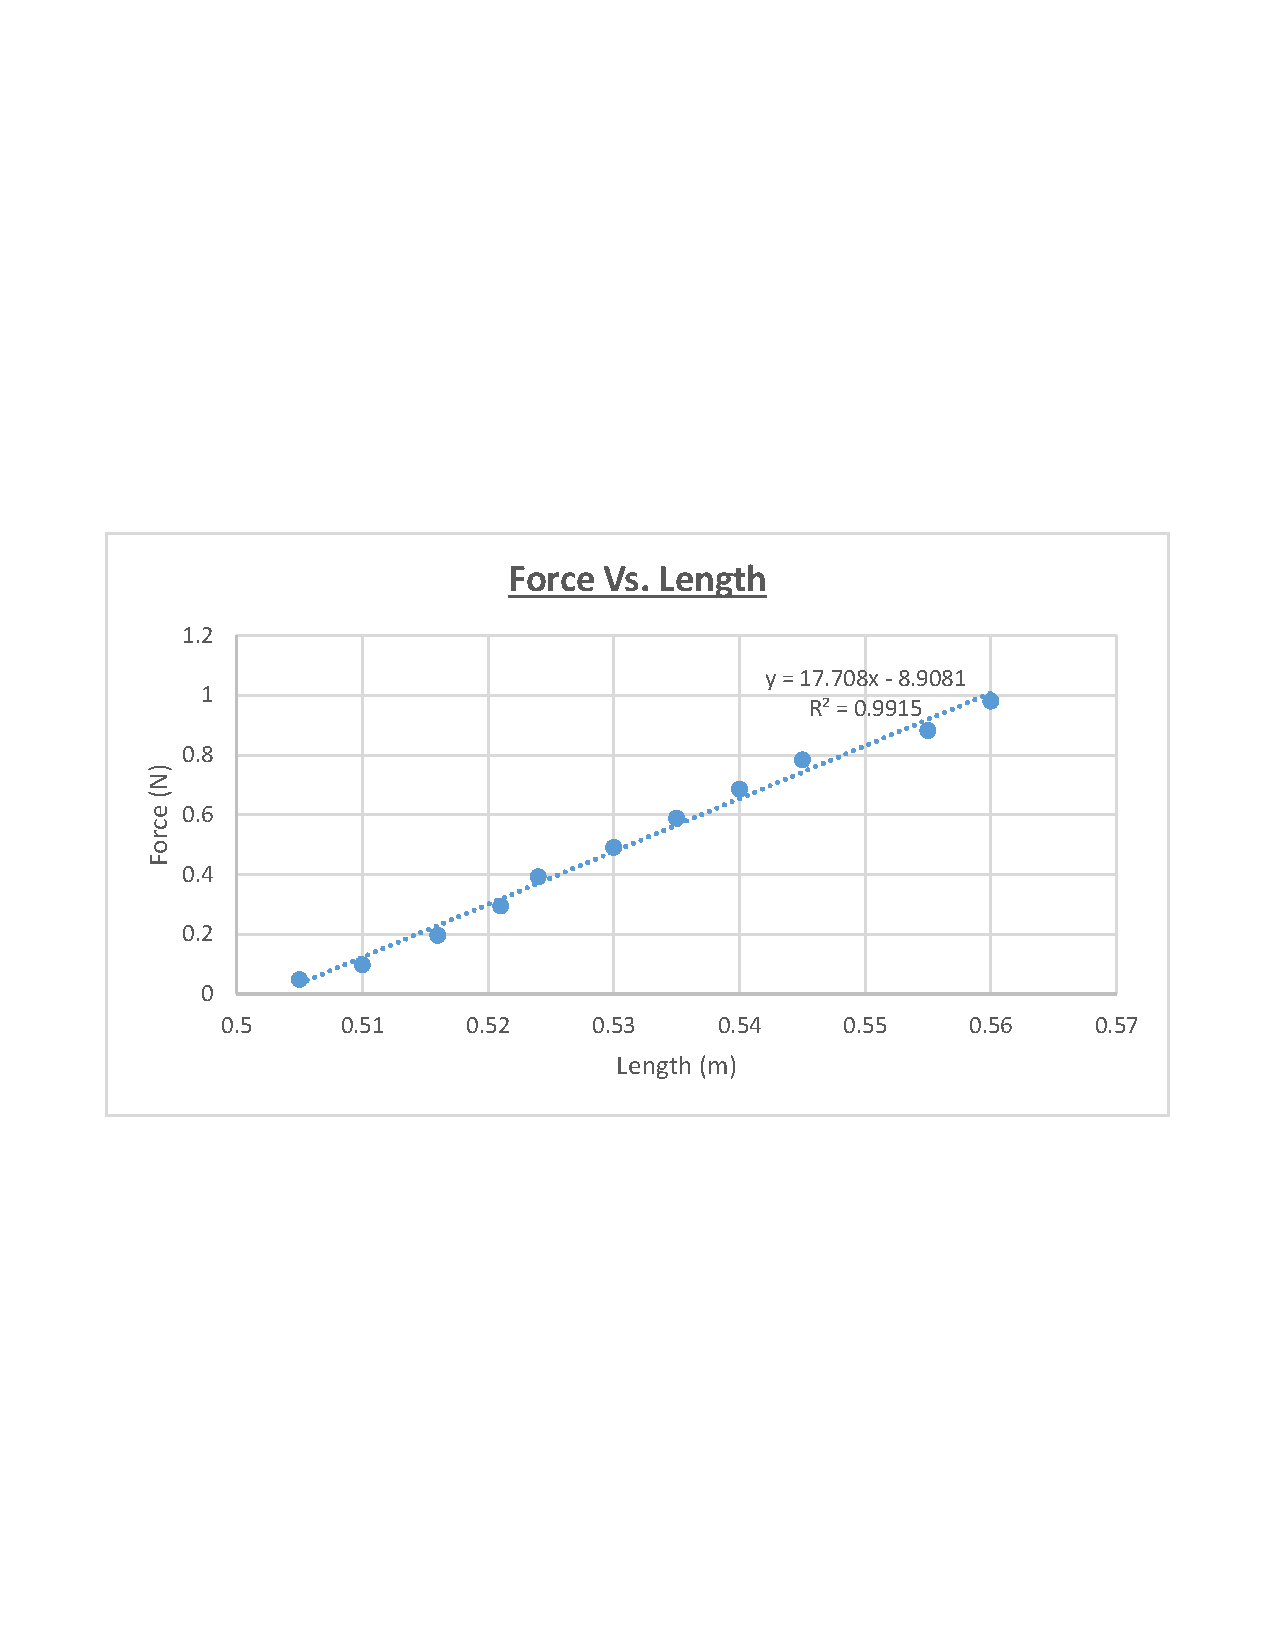
\includegraphics[width=5in]{P6Lab10Data.pdf}\\
\vspace{-50mm}
\textit{Figure 1: Force Vs. Length graph that models Hooke's law. The slope of the trendline created by the data is the k, spring constant, of the rubber bands}
\end{center}

Shown in the Figure 1, the k value of the rubber bands is approximately 17.708$\frac{N}{m}$.

To find $y_0$, the equilibrium length of the rubber band with no masses on it, is the value of x in the linear equation y = 17.708x - 8.9081, when y = 0N; when there is no mass pulling on the rubber bands. Therefore, we get that $y_0 = .5031m$. Adding this value with the length of the 100g mass, will give us $y_0^*$; when added together $y_0^* = 0.5612m$. 

\subsection{Calculating $y_f$ and the Final Result}

Recall that in the quadratic equation a = k, b = -2(mg + k $y_0^*$), and c = k$y_0^{*2}$. Now that we know what k is, from the slope of the trendline in figure 1, and what $y_0^*$ is from the previous section, $y_f$ can be calculated. Since the quadratic equation was used, there will be two answers for $y_f$ one from the positive root and the other from the negative root. When the quadratic is solved, two values are obtained: $y_f =$ 0.872m (positive root), 0.361m (negative root). For the purpose of this experiment, we will use the positive root as the distance away from the box on the ground to safely tap the box. 

When tested the 100g mass didn't hit the ground, and lightly tapped the box! 

I believe that the value, given by the negative root, is the height that the box "jumps" back up to, after reaching the maximum stretch.  

\section{Discussion} 

The height of $y_f$ was successful in causing the mass to lightly tap the box! It was imperative to not stretch the rubber band too much, so the material properties of the rubber band don't change too much. That's why it was important to obtain a successful run on the first try, or the calculations might become messed up from the constant stretching of the rubber band. 

The experiment utilized the quadratic equation to obtain the value of $y_f$, the positive root value was the value used in the experiment to lightly tap the box. The negative root value in the experiment was the height in which the box "jumps" back up from the maximum stretched length and compresses to the negative root height value.

\section{References}

\hspace{-6.5mm}
Leap of Faith Bungee Jumping Physics 06 Lab, Dr. Melanie Lutz\\



\end{document}
